\section{The Architecture}

This project has been implemented using ROS framework. It is a modular application that enables other nodes to query and interact with the knowledge base. An external interface node allows several operations including the export of the Assertion Box. Four nodes are involved in this application and the communication between them relies on an inter-process protocol handled by ROS.

\subsection{System description}
In the following subsection, the implemented nodes and their interaction with the system will be discussed. 

\begin{figure}[H]
\centering
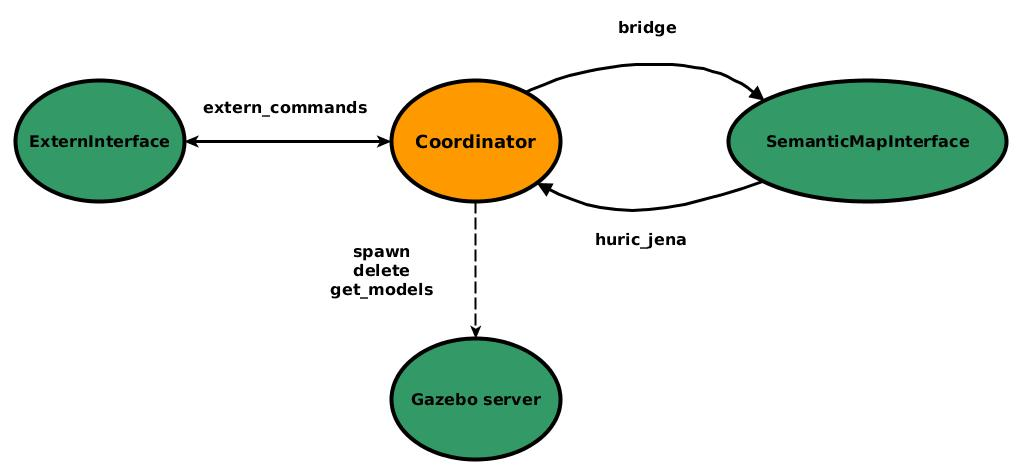
\includegraphics[width=0.8\textwidth]{imgs/arch1.jpg}
\label{fig:actions}
\caption{System Architecture}
\end{figure}

\subsubsection{SemanticMapInterface Node}
The knowledge base is loaded from the SemanticMapInterface which is a Java node based on the Jena Ontology API. This process allows requesting nodes to access and manipulate the ontology using a predefined set of operations.

\begin{figure}[H]
\centering
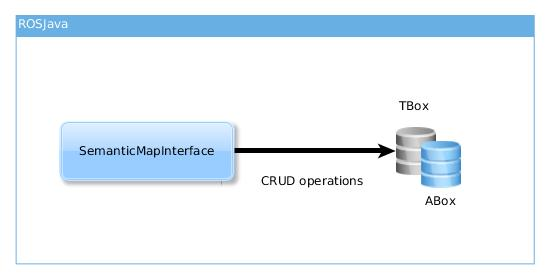
\includegraphics[width=0.8\textwidth]{imgs/semantic.jpg}
\label{fig:actions}
\caption{SemanticMapInterface Node}
\end{figure}

The exposed operations include:

\begin{itemize}
\item Loading the Terminology (TBox) and Assertion Box (ABox) into memory,
\item Listing instances, their spacial properties and their preferred lexical reference,
\item Adding a new entity of a particular class, with the spacial and lexical properties specified as arguments,
\item Updating properties of active entities,
\item Removing active entities,
\item Invoking OWL-FULL reasoner and performing inference operation given a domain model, 
\item Exporting in OWL format the list of instances present or the augmented ABox with derived properties.

\end{itemize}

\subsubsection{Gazebo Nodes}

Gazebo is a free (freedom) and open source robot simulation environment. It provides high performance physics engines to model real world dynamics, render 3D objects and environments. The Gazebo server \textit{gzserver} executes the simulation process including physics updates. The Gazebo client runs the UI and provides a 3D environment and handy controls to modify simulation properties. These nodes provide a set of ROS API's that allows users to modify and get information about various aspects of the simulated world.

Topics can be used to set the pose and twist of a model by publishing desired model state message to /gazebo/set\_model\_state\_topic. It is possible to retrieve model and link states using Topics. Gazebo publishes /gazebo/link\_states and /gazebo/model\_states\_topics, containing pose and twist information of objects in simulation with respect to the gazebo world frame. Services can be used to create/spawn and destroy models dynamically in simulation.

\subsubsection{Extern Interface Node}
This node has been implemented to test the required specifications. It simulates external requests by publishing predefined encoded messages on a topic to which the Coordinator is subscribed. The supported operation are listed in section \ref{sec:objectives}


\subsubsection{Coordinator Node}
The Coordinator node is a python script that performs several actions and communicates with other nodes in the system. One responsibility of the coordinator is to keep track of instances and trigger update requests when a 3D model is manually grabbed and moved in the simulation. This node provides a dynamic rooting of requests from the External Interface node to the ontology handler or Gazebo. 

Basic operations include:

\begin{itemize}
\item Handles high level requests from other nodes such as visualizing or exporting the  list of instances present in the ontology.
\item Tracks 3D absolute positions of objects in the simulation,
\item Notifies the ontology manager that an instance's property has changed,
\item Forwards 3D spawn and delete task to Gazebo,
\item Ensures consistency between the Assertion Box and the simulated world.
\end{itemize}

\subsection{Test cases}

The following test cases have been performed:

\begin{itemize}
\item Initialization from non empty ontology (TBox and ABox),
\item Retrieve collection of instances and render 3D models in Gazebo,
\item Request a detailed list of properties about active entities,
\item Manually drag objects in scene and sync new properties with the ABox,
\item Request Instances enumeration from ExternalInterface,
\item Perform a consistency check.
\item Requests:
	\begin{itemize}
		\item Deletion of entities,
		\item Insertion of default instance,
		\item Insertion of instance with specified type, spacial and lexical property,
		\item Export to specified file.
	\end{itemize}
\end{itemize}